\documentclass{article}

% Packages
\usepackage[utf8]{inputenc}
\usepackage{amsmath}
\usepackage{listings}
\usepackage{algorithmicx}
%\usepackage{algorithm}
\usepackage{algpseudocode}
\usepackage{hyperref}

\makeatletter
\def\BState{\State\hskip-\ALG@thistlm}
\makeatother

\title{Algorithm Description}
\author{ Group 6 (Ross Chadwick, Eirik Kultorp, Milan Blonk) }
\date{Heuristics January 2017}

\usepackage{natbib}
\usepackage{graphicx}

\begin{document}


\maketitle

\section{Introduction}

We will implement \href{https://en.wikipedia.org/wiki/Simulated_annealing}{Simulated Annealing} (hereby SA) as our optimisation algorithm to seek good solutions AmstelHaege assignment. This algorithm is generally suitable for approaching a global optimum, which in our context is a plan of maximal value, as determined by Groundplan().getPlanValue() in the provided environment. The features of SA are in contrast with greedy algorithms such as hill climbing, which tend to get stuck in local maximum while often missing the global maximum when there are many peaks, which is the case for our problem - we expect a large spread of possible (near) optimal solutions. 

\section{Problem Description}

\subsection{Informal description}

A new residential area, 'AmstelHaege', has to be developed. This residential area has to contain family homes, bungalows, mansions type of houses, playgrounds and surface water. For a plan to be valid it has to hold for some constrains. First, the plot is a 200x170 meter area. Second, a total of 20 percent of the area has to be surface water. Third, the surface water has to be contained in at most four bodies of water with side ratios of 1:4 which may not be adjacent and need at least 3 meters between them. Four, the houses have to be present in a ratio of 5:3:2 respectively. Fifth, each house needs to have some free space around it called clearance. Sixth, each house is no more than 50 meters away from a playground. Lastly the family homes need 2 meter clearance, bungalows 3 meter clearance and the mansions 6 meter clearance between them. Plans varying a total of 40, 70 and 100 houses are considered. Besides this assignment an advanced assignment is given where an optimal number of houses (with and without playgrounds) if no restrictions hold for the numbers per type. That is, any type can be used or not.

The plans constructed will be valued by the given getPlanValue function that values the plans. This function takes factors as housing value, which increases with clearance, and playground costs into account and produces a single output number resembling the value of the plan. The goal for the (advanced) assignment is to set up an algorithm that provides an good approximation to the maximum valued plan that is valid. To achieve this an algorithm has to be set up that configures placement of all elements in the plan in a way that gives a good global solution.

\subsection{Formal description}

Element classes WB, PG, and R1, R2, R3 are defined as rectangles of different dimensions. FH, B and M are subclasses of R. The elements are placable on a 2D grid of a fixed size. PGs have negative value, WB has 0 value, and RX elements have different positive constant values plus a value determined by the distance to the nearest other R element. No elements may overlap, and R elements must be within a certain range of a PG. Our task is to place N RX elements on a 2D grid in such a way as to maximize the sum of all the elements' values, while also respecting the constraint of R type proportions (i.e. a*R1,b*R2,c*R2).

\subsection{State Space}

The state space is continuous, with an infinite number of possible states. 

\subsection{Correct and Optimal Solutions}

Correct solutions are easily brute forceable. Optimal solutions are not feasibly brute forcable. An optimal solution is a configuration for which no other configuration has a higher value. 

\section{Algorithm}

\subsection{Description}

SA is a probabilistic method of finding a global optimum in a state space. SA algorithms have a generic top layer, common for all problems. In our work we tailor SA to our specific needs with heuristics to determine which moves to make, moving from one state to another. 

We will apply SA to perform different tasks: 

\begin{enumerate}
    \item Initial placement of water and playgrounds, optimizing for area on which we can place residences
    \item Placement of residences, optimizing for plan value.
\end{enumerate}  

The second application will take the output of the first application as input, determining the initial state. The two stages are very similar, in the sense that they both use SA. They vary by what value they optimize for and what elements are placed. 

Our SA algorithm will be expanded with various parameters as we go. Below is the basic skeleton of how we intend to start the implementation. \\ For example, we plan to implement and chage the parameters of the goal (Upper limit), getNeighbor() function, acceptance probability function, initial temperature and temperature scheduler function.% todo split up, put parts in experimental conditions section

\subsubsection{generateNeighbor()}

The generateNeighbor() function is used to create a new state based on a seed state - defining a \textit{move}. It should not be deterministic, as different states generated from the same state will be compared to the seed state. It is within the generateNeighbor function that heuristics become important. We can try using the temperature as a factor in the randomness of the generated states. We will do an empirical evaluation of how useful this is.

\subparagraph{Possible moves}

A move may include any/all of the following actions:
\begin{itemize}
    \item Moving an element
    \item Swapping positions of elements  
    \item Flipping an element
\end{itemize}


\paragraph{Water and Playground Placement Stage Heuristics} 

We want as few playgrounds as possible (because playgrounds have negative value), while their radiuses cover as much area as possible (because all residences must be within range of a playground). We also want as little water as possible (because they have no value but take up space that could be covered by playground range). Water placed near a map edge but not touching it in such a way that no residences can be fitted between it and the edge also implies wasted space. Playground range overlapping water and reaching outside the map is also wasted space. 

\paragraph{Residence Placement Stage Heuristics}

We will apply different heuristic functions to determine what moves to make. These functions should be local to where we apply the change, as on this level we are making small changes in the hope that it will increase the global value. But we will not directly use the getPlanValue() function at this point, as this is being done on the above layer (in the main SA function), and it would undermine the use of heuristic functions at this point.
\\
\\
Some heuristics that we will consider are:
\begin{itemize}
 \item Maximize clearance from other residences. 
 \item Prioritise clearance of the most valuable house type (house price divided by house area)
\end{itemize}

To be expanded. 

% To avoid getting stuck near a local optimum, the resulting state must be far enough away from the seed state to escape the local optimum. To avoid missing out on the global optimum when near it, it must not always move far away. Thus, a factor that influences distance from the seed must be included. It should be random, so there is variance in the seed-child distance. This should ensure that the algorithm both zooms in on local optimums, and jumps far and approaches a better state than the local optimum. 

\subsection{Pseudo Code}

\subsubsection{Simulated Annealing Variations}
Below are the basis of our algorithms. They pseudo code will likely not reflect the end solution and we will be experimenting and expanding as we gather results.
\\
    \begin{algorithmic}
        \State $\textit{MAX\_STEPS} \gets \text{ 1000 // we will vary this }$
        \State $\textit{state} \gets \text{ plan.deepCopy() }$\\
            \Procedure{simulatedAnnealingValue}{$state$}   
            \For{$step\gets 1, MAX\_STEPS$}
                \State $t \gets temperature(step/MAX\_STEPS)$
                \State $neighbor \gets getNeighbor(state)$
                \If{$acceptanceThreshold(state.planValue(), neighbor.planValue(), t) >= random()$}
                    \State $t \gets temperature(step/MAX\_STEPS)$
                \EndIf
            \EndFor
            \State \textbf{return} $state$
            \EndProcedure
            \\
            \Procedure{simulatedAnnealingArea}{$state$}   
            \For{$step\gets 1, MAX\_STEPS$}
                \State $t \gets temperature(step/MAX\_STEPS)$
                \State $neighbor \gets getNeighbor(state)$
                \If{$acceptanceThreshold(state.placeableArea(), neighbor.placeableArea, t) >= random()$}
                    \State $t \gets temperature(step/MAX\_STEPS)$
                \EndIf
            \EndFor
            \State \textbf{return} $state$
            \EndProcedure
    \end{algorithmic}

\subsubsection{getNeighbor() Variations}
    \begin{algorithmic}
            \Procedure{getRandomNeighbor}{$state$}
            \State $residence \gets state.selectRandomResidence()$
            \If{$random() < 0.5$}
               \State residence.moveInRandomDirection()
            \Else
                \State state.swap(residence, state.getRandomResidence())
            \EndIf
            \State \textbf{return} $state$
            \EndProcedure
    \end{algorithmic}

\pagebreak


The diagram below visualises the core concepts of our description in the previous section. 

\begin{figure}
\subsection{Flowchart}
  \makebox[\textwidth][c]{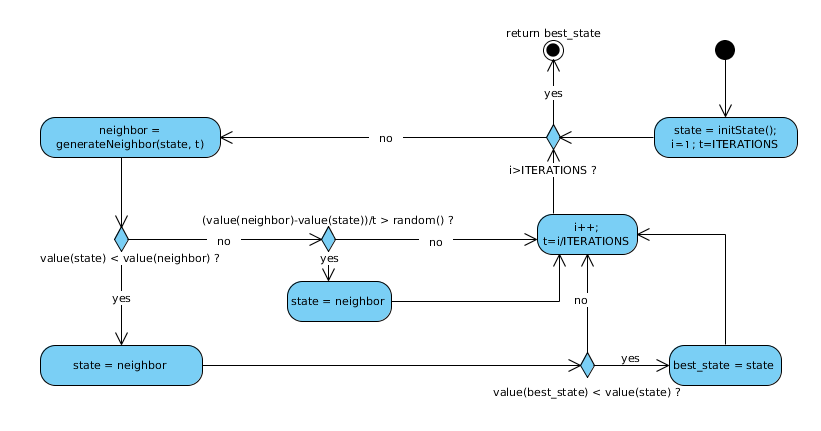
\includegraphics[width=1.5\textwidth]{diagram.png}}
  \caption{Simulated Annealing Flowchart.}
  \label{fig:flowchart}
\end{figure}

%\pagebreak

\section{Difficulties, limitations, restrictions}

\subsection{Ambiguity in assignment details}

The assignment states several contradicting situations regarding clearance. At first is stated that 'a playground does not count as clearance', this means two houses could not be placed opposite sides of a playground without clearance to the playground. The assignment however also states that 'The clearance of a home is the smallest distance between it and the closest other home', this means that two houses could be placed opposite sides of a playground without clearance to the playground as the playground is functioning as distance between the two houses.

In the advanced assignment it is asked for to 'find the optimal number of houses (with and without playgrounds) if no restrictions hold for the numbers per type. That is, any type can be used or not'. This can be interpreted in two ways. The first interpretation is that the constraint regarding the ratio of different houses is left intact but some types may be left out. The second interpretation is that the ratio of houses is discarded and any number of houses of types can be used.

\subsection{Incompleteness of given code}

The given code had a large amount of bugs which we had to resolve. This took up quite an amount of our productive time. The bugs also delayed our decision making and algorithm design as in many cases, we had to go back and question the guidelines, attempting to implement them as best as we could interpret them. This led to quite a few revisions of our analysis of the problem.

\section{Experimental setup}

\subsection{Algorithmic Variants}

Different versions of generateNeighbor(), implementing different heuristics within each. See generateNeighbor section above for more details. Different sets of generateNeighbor() functions will be used for the first (pg/wb placement) and second (residence placement) stages. 


\subsection{Experimental Conditions}

We will run the experiment with different values for max\_iterations, and with different generateNeighbor() algorithms that SA will be using to find the next housing location, and observe the results. 

\subsection{Problem Instances}

Problem instances are as defined by the assignment: ratio of 5:3:2 FamilyHouses:Bungalows:Mansions, on a grid of 200x170 distance units, with a total of 40, 70 and 100 residences in different instances. 

\subsection{Benchmarking}

We will compare our results for this SA algorithms with each other across the different variants, changing one variable at a time in a systematic way. We will also benchmark our SA variants against previous implementations of any algorithms available online, and against a evolutionary algorithm we implemented. 

\subsubsection{Intelligent vs SA Placement of Water and Playgrounds} % ?

During our analysis of the given problem, we also came up with a deterministic approach to dynamically (and statically) placing water and playgrounds. This was done as an experiment and will also be used to evaluate SAs solutions for water and playground placement. The dynamic approach first places the required water with number of bodies as a parameter. The total usable area left is then divided by the reachable area of a playground and either the floor() or ceil() integer value of this calculation is used as the number of playgrounds to place in a matrix-like format.
\\
On the next pages are some screenshots visualising our placements so far. 


\begin{figure}
  \makebox[\textwidth][c]{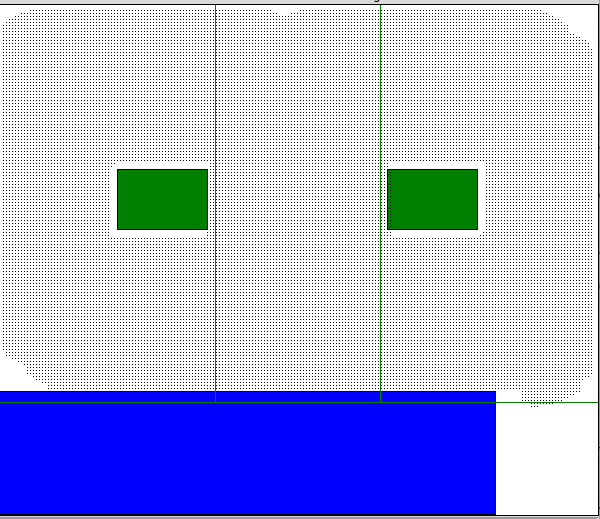
\includegraphics[width=1.2\textwidth]{DistrictPlanner.png}}
  \caption{A screenshot of our dynamically placed water and playgrounds (With visualised effective radius). Has coverage 0.6836 }
  \label{fig:Dynamic Placement}
\end{figure}

\begin{figure}
  \makebox[\textwidth][c]{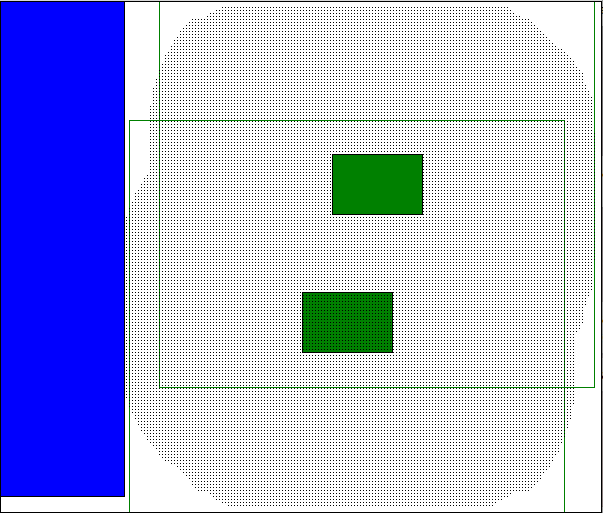
\includegraphics[width=1.2\textwidth]{Vertical.png}}
  \caption{A screenshot of an attempt at manually placing the elements. Has coverage 0.6829}
  \label{fig:Dynamic Placement 2}
\end{figure}

% During our placeable area optimisation stage, we will vary the heuristics function, which uncludes varying transformative metrics such as the spread of playgrounds from the origin, the number of water bodies and their locations

\end{document}
